\thispagestyle{quantoannone}
\pagestyle{quantoan}
\everymath{\color{quantoan}}
\graphicspath{{../quantoan/pic2/}}
\blfootnote{\color{quantoan}$^1$Viện Vật lý.}
\begingroup
\AddToShipoutPicture*{\put(0,616){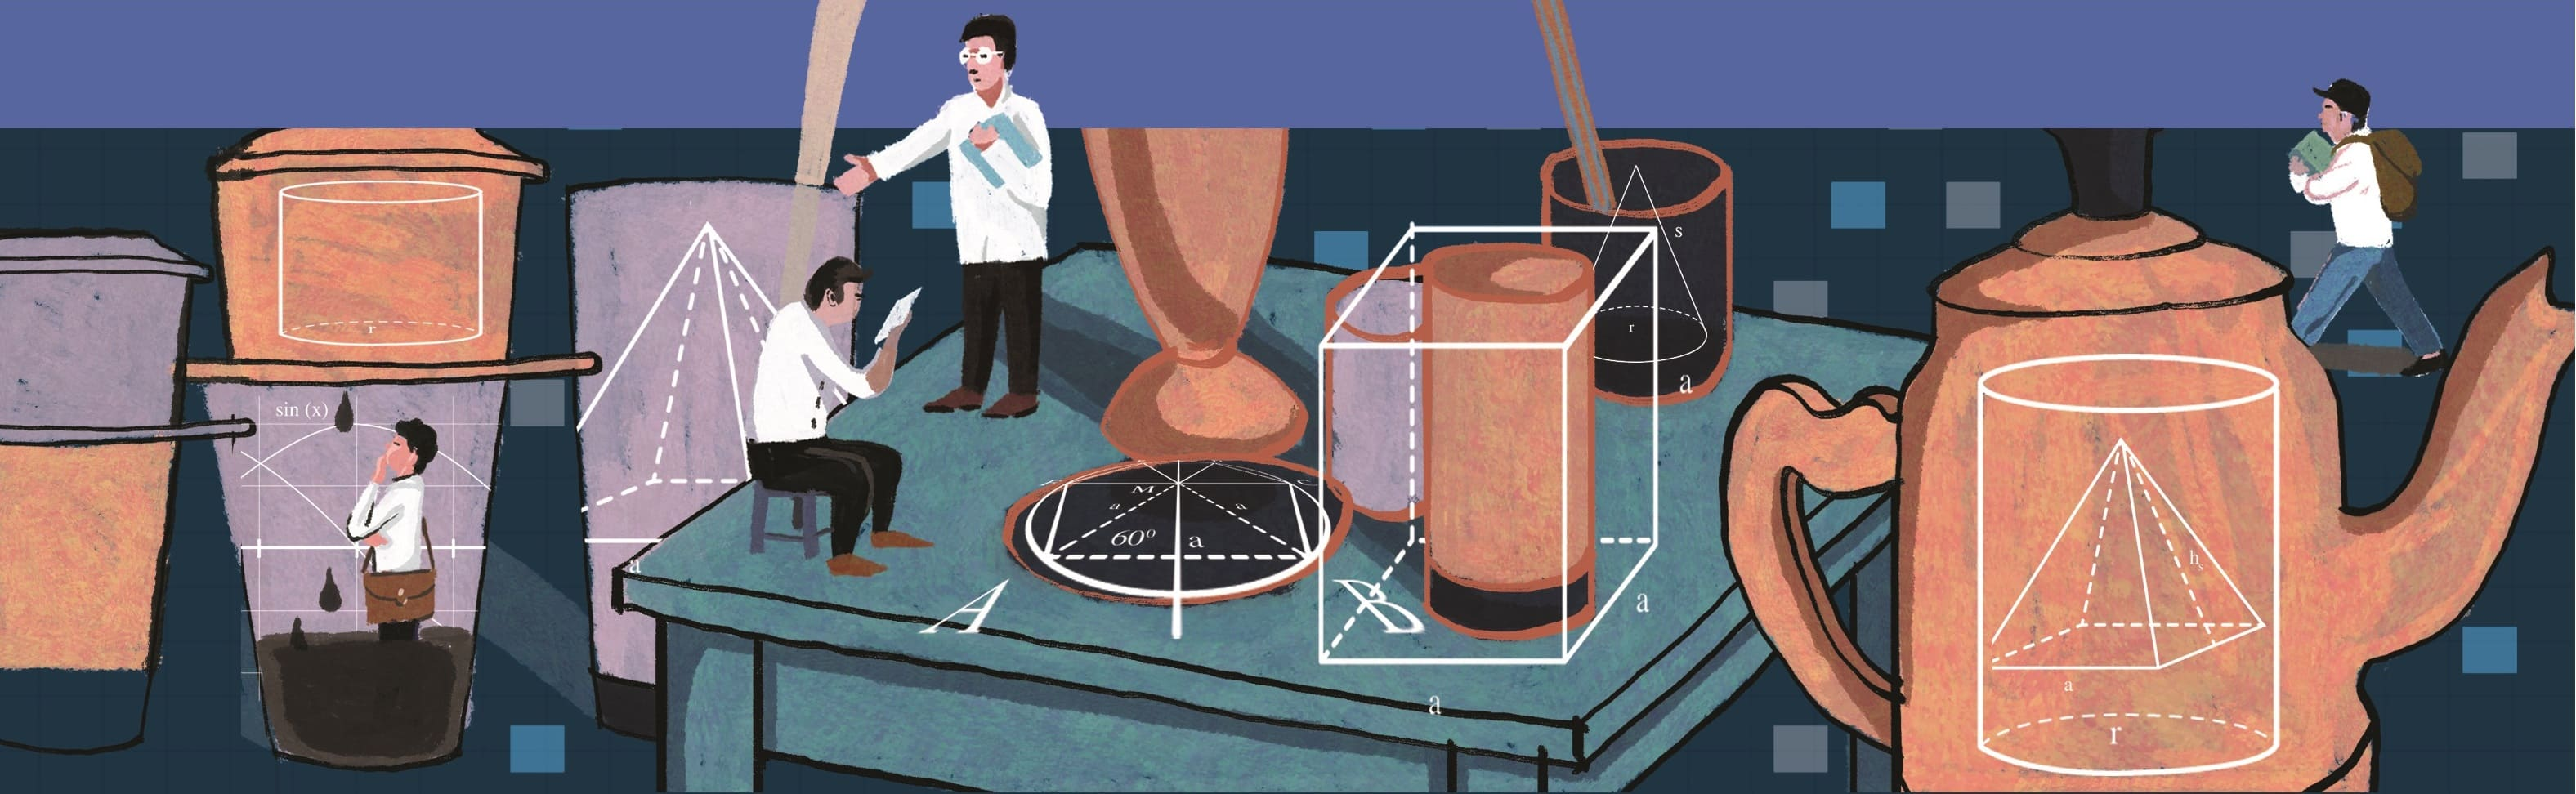
\includegraphics[width=19.3cm]{../bannerquantoan}}}
\AddToShipoutPicture*{\put(132,550){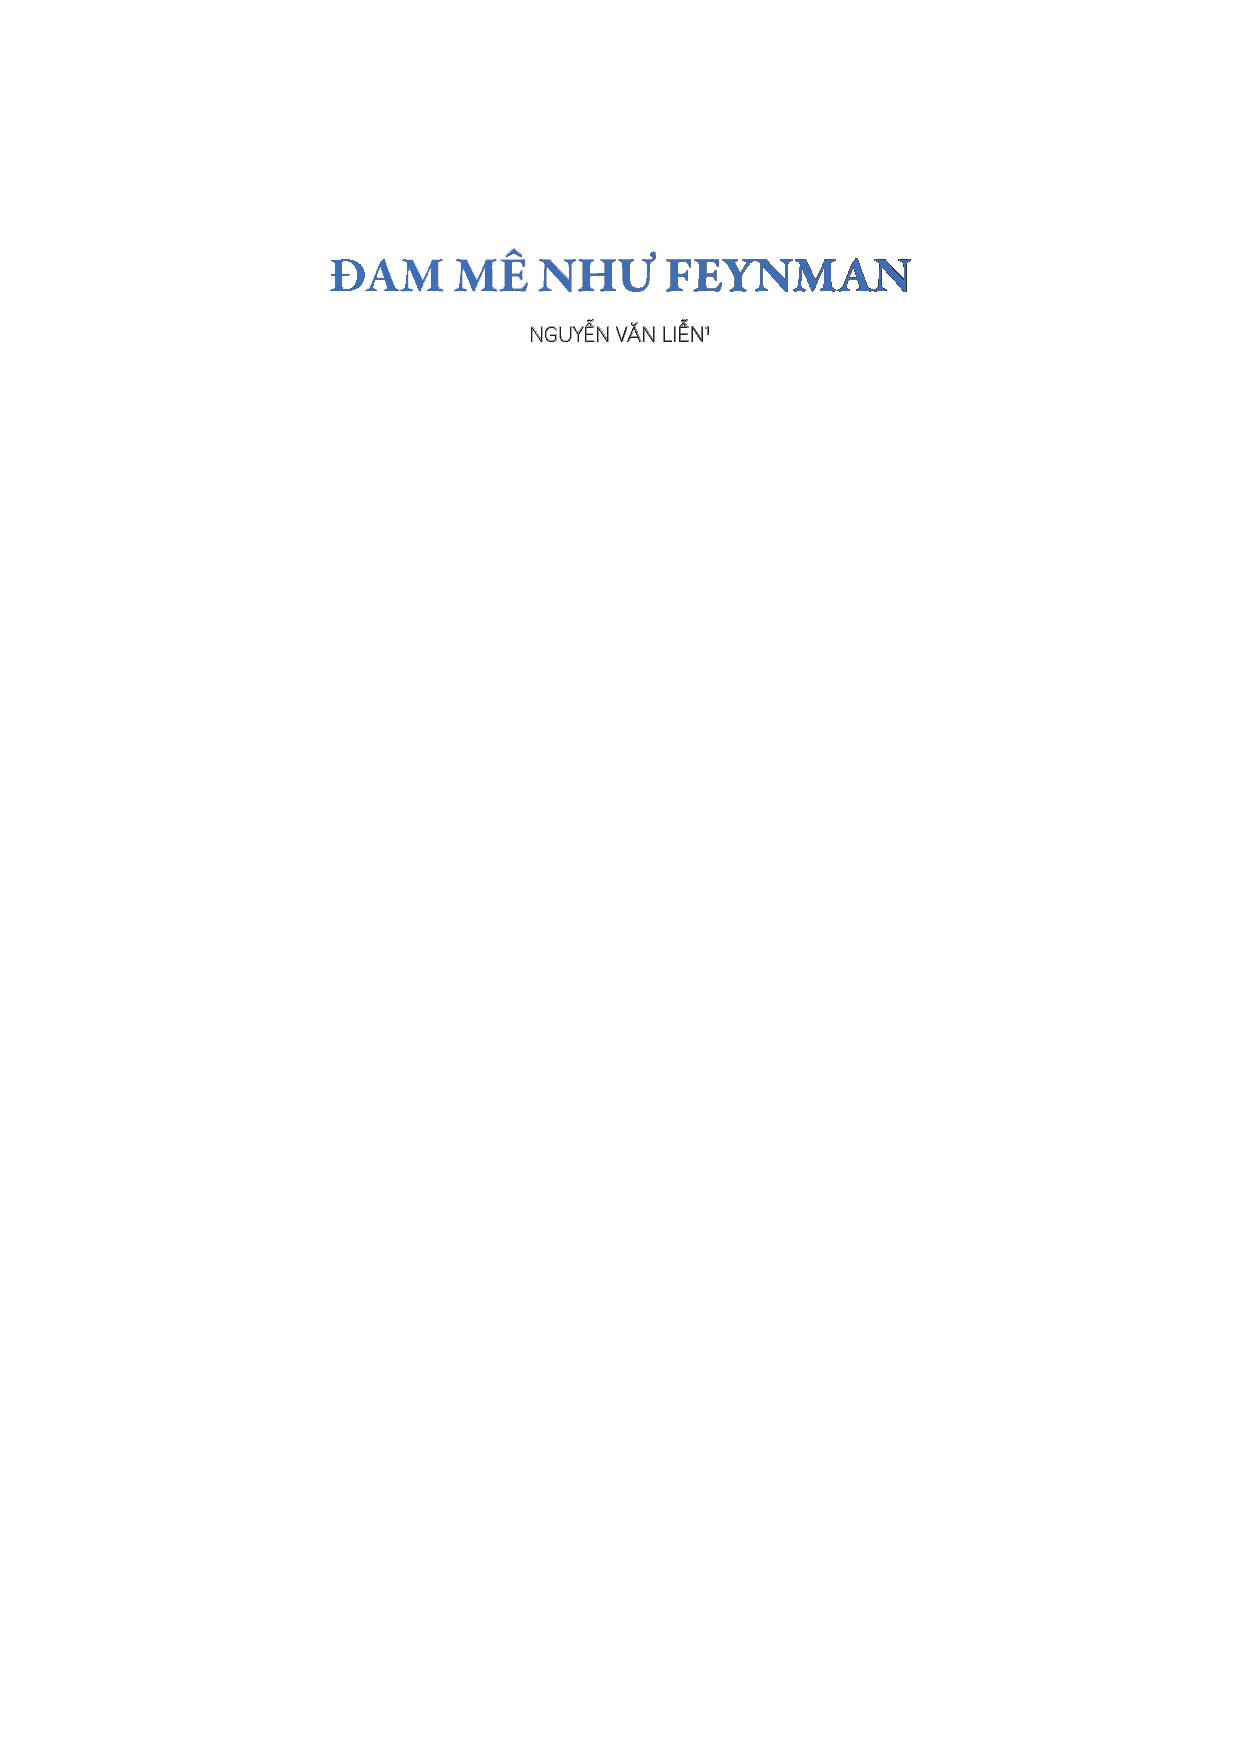
\includegraphics[scale=1]{../tieude2.pdf}}}
\centering
\endgroup
\vspace*{160pt}

\begin{multicols}{2}
	Richard Feynman ($1918-1988$, Mỹ) nổi tiếng là người trung thực không khoan nhượng và đam mê đến tận cùng. Về tính trung thực, người ta hay nhắc đến vụ ông trình diễn trực tiếp trên TV một ``thí nghiệm nhỏ", bỏ vòng cao su vào cốc nước đá, minh chứng rằng cao su mất tính đàn hồi ở nhiệt độ thấp, qua đó chỉ ra nguyên nhân dẫn đến thảm họa tàu vũ trụ con thoi ``Challenger", vạch trần chiến dịch tung hỏa mù của NASA về nguyên nhân của thảm họa này. Để công bố với người dân Mỹ sự thật ấy, Feynman đã phải vượt qua sức ép khủng khiếp từ các cơ quan công quyền Mỹ, trong đó có CIA và NASA. 
	\vskip 0.1cm
	Feynman lắm đam mê. Đam mê vật lý, Feynman nhận giải Nobel Vật lý năm $1965$. Đam mê chơi trống, vở ba--lê do ông đệm trống nhận giải nhất trong cuộc thi ba--lê toàn nước Mỹ và giải nhì trong cuộc thi quốc tế tại Paris. Đam mê vẽ, ông đã có triển lãm tranh riêng. Không rõ ông biết những ngôn ngữ nào, chỉ biết thăm Brazil ông dạy bằng tiếng Bồ, thăm Nhật ông giao du bằng tiếng Nhật. Rồi có lần bạn bè định ``cho ông một vố", họ nhờ một cô Hoa kiều đón tiếp ông bằng tiếng Trung, Feynman đáp lại và cô ấy kêu trời, vì ông nói tiếng Quảng Đông, còn cô chỉ nói tiếng Bắc Kinh. Rất nhiều ``đam mê" kiểu như vậy được kể trong cuốn ``Feynman, chuyện thật như đùa" (NXB Trẻ) và hầu như tất cả đều có kết cục mỹ mãn, kiểu như giải Nobel. Có thể bạn nghĩ chắc ông này ``con nhà nòi", học ``trường quốc tế" từ nhỏ! Xin thưa, bố của Feynman là người bán rong bán quần áo, còn mẹ thì nội trợ. 
	\begin{figure}[H]
		\vspace*{-5pt}
		\centering
		\captionsetup{labelformat= empty, justification=centering}
		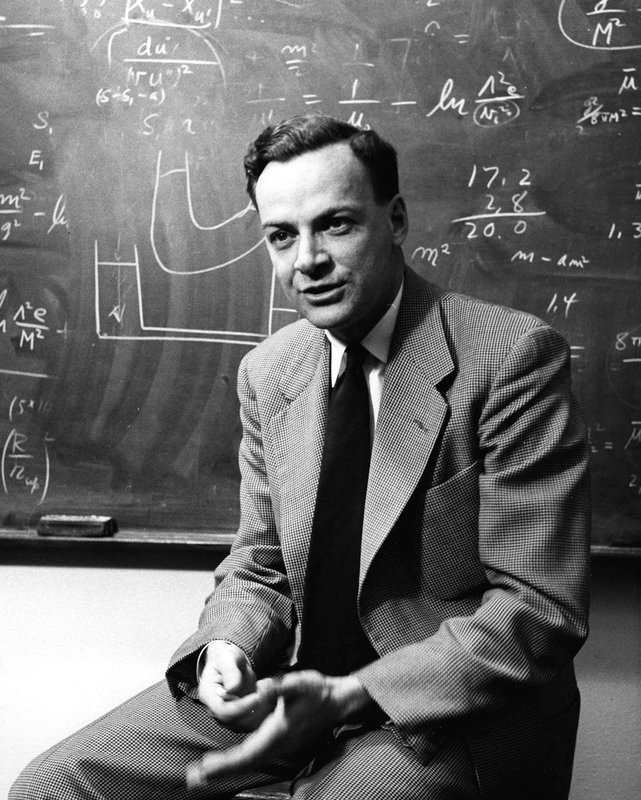
\includegraphics[width= 1\linewidth]{1a}
		\caption{\small\textit{\color{quantoan}Richard Feynman (ảnh từ bộ sưu tập của Viện Công nghệ California -- CalTech).}}
		\vspace*{-10pt}
	\end{figure}
	Ông chơi trống bongo cực giỏi, nhưng chưa bao giờ học nhạc lý. Ông vốn vẽ rất kém, tự nhận chẳng thể vẽ nổi cái gì ngoại trừ cái kim tự tháp chỉ gồm mấy đường thẳng. Để học vẽ, Feynman ``đổi công" với một họa sỹ: ông dạy vật lý cho họa sỹ còn họa sỹ dạy vẽ cho ông. Hãy tưởng tượng một giáo sư nổi tiếng thế giới ngồi trong lớp vẽ cùng các cháu $8-9$ tuổi học cách gọt bút chì. Đam mê như thế chỉ có ở Feynman. Và, với ông đam mê chính là nguồn cội của thành công, chứ chẳng phải ``con nhà nòi" hay ``trường quốc tế" nào cả. Tiền bạc và chứng chỉ đầy người, mà không đam mê gì, thì làm sao có thành quả! 
	\begin{figure}[H]
		\vspace*{-5pt}
		\centering
		\captionsetup{labelformat= empty, justification=centering}
		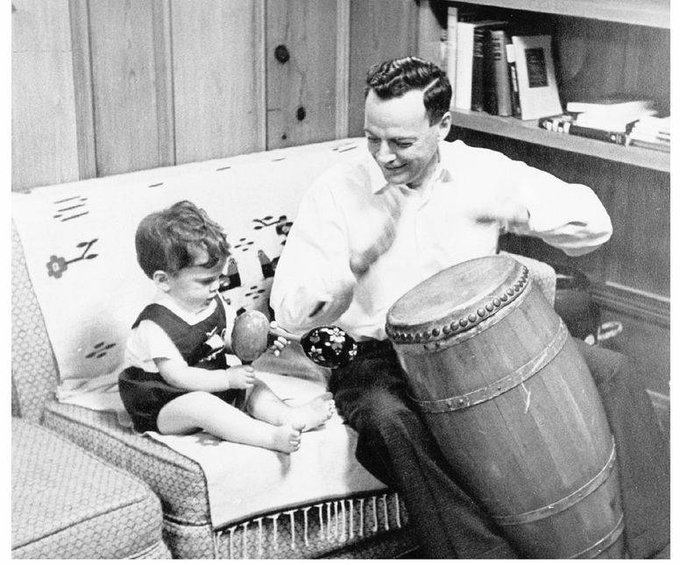
\includegraphics[width= 1\linewidth]{2a}
		\caption{\small\textit{\color{quantoan}Feynman chơi trống bên con trai (ảnh từ Internet).}}
		\vspace*{-10pt}
	\end{figure}
	Duy có đam mê cuối cùng, Feynman đã không kịp nhìn thấy những gì mình muốn, trước khi về cõi vĩnh hằng. Đó là ``Cuộc phiêu lưu cuối cùng của Feynman"\footnote[2]{\color{quantoan}Xem thêm: Cuộc phiêu lưu cuối cùng của Feynman, in lần $2$, NXB Trẻ, $2023$.}. Cuộc phiêu lưu khởi đầu bằng một con tem có xuất xứ từ một nơi gọi là Tannu Tuva, mà Feynman có được từ khi còn nhỏ. Cái tên ``Tuva" xa lạ nằm yên trong đầu Feynman, cho đến một ngày hè $1977$ nó trở thành mục tiêu cho ``cuộc phiêu lưu" kéo dài hơn $10$ năm cuối của cuộc đời ông. Tôi cược là nhiều bạn chưa biết Tuva là địa danh nào và ở đâu. Để đỡ tra cứu, xin ``bật mí" ngay: đó là tên một quốc gia nhỏ nằm giáp phía Tây Bắc của Mông Cổ, vốn độc lập, nhưng đã sáp nhập vào Liên Xô cũ (và Nga ngày nay). Thủ đô của Tuva là Kyzyl. Tuva có gì đặc biệt mà khiến Feynman mê mệt đến vậy?
	\vskip 0.1cm
	Bạn có biết đâu là trọng tâm của châu Á (lục địa thôi chứ không tính các đảo)? Lấy tấm bìa cứng phẳng, vẽ lên đó bản đồ châu Á, cắt theo đường biên để được miếng bìa hình châu Á lục địa. Dùng một chiếc bút đầu nhọn chống phía dưới tấm bìa, di di đầu bút, để tìm vị trí mà tấm bìa nằm cân bằng trên chiếc bút thẳng đứng. Vị trí đó rơi vào Kyzyl, trọng tâm của châu Á. Tất nhiên, các nhà khoa học xác định điểm này bằng các phương pháp chính xác hơn, và ngày nay ở Kyzyl có tấm bia lớn khẳng định vị trí đặc biệt của thành phố này. Nhưng, chỉ chừng ấy thì không đủ để Feynman mất tới cả chục năm tìm cách tới thăm Tuva.
	\begin{figure}[H]
		\vspace*{-5pt}
		\centering
		\captionsetup{labelformat= empty, justification=centering}
		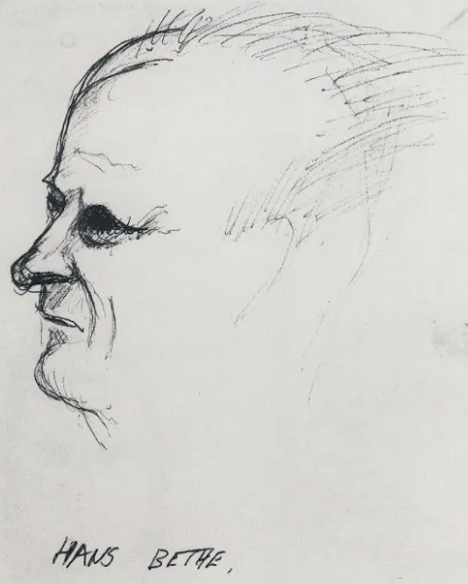
\includegraphics[width= 1\linewidth]{3a}
		\caption{\small\textit{\color{quantoan}Feyman vẽ Hans Bethe (giải Nobel Vật lý $1967$).}}
		\vspace*{-10pt}
	\end{figure}
	Cái chính là ở quốc gia tí xíu bao bọc bởi những dãy núi cao ấy, thời gian gần như ngừng trôi: tất cả vẫn nguyên sơ như $500$ hay $1000$ năm trước. Thảo nguyên hoang dại. Những đàn tuần lộc hay bò Tây Tạng cũng dường như hoang dại. Cuộc sống du mục không thể tự nhiên hơn. Một nền văn hóa xa xưa và kỳ thú với kiểu hát hai giọng chỉ có ở Tuva, với thứ văn tự không thể tìm thấy trong bất cứ tự điển nào, với các tập tục rất lạ điều hành bởi các tù trưởng uy nghi và bí ẩn v.v. Tiếc là ít người biết Tuva, chứ không, người ta đã gọi quốc gia này là ``Thảo nguyên Xanh" cuối cùng của hành tinh Trái Đất (như Congo là Hành tinh Xanh cuối cùng). Đam mê Tuva, Feynman tìm đọc mọi tài liệu về Tuva, tìm hiểu văn tự Tuva, học cách hát của dân du mục Tuva, ăn mặc và trang trí như tù trưởng Tuva \ldots Và, nhất là, ông tìm mọi cách để có thể đến thăm Tuva.
	\vskip 0.1cm
	Đó là thời Chiến tranh Lạnh, lại nghe nói, gần Tuva có một cơ sở nghiên cứu bom nguyên tử, nên nơi đây là ``vùng cấm" với khách du lịch, nhất là khách nước ngoài. Thực ra, Viện Hàn lâm Khoa học Liên Xô sẵn sàng mời Feynman sang Moscow  đọc bài giảng rồi đi ``tham quan Kyzyl" theo kiểu mặc com--lê ở khách sạn có người bảo vệ v.v. Nhưng Feynman không thích như vậy, mà muốn tự mình mang ba--lô đến thảo nguyên, ngủ lều, uống sữa tuần lộc và hát hai giọng cùng dân bản xứ. Ấy thế cho nên ông mất cả chục năm tìm kiếm một giấy mời như mình muốn. Và, đầu tháng Ba $1988$, một giấy mời như thế đã gửi đến địa chỉ của Feynman, chỉ tiếc là hai tuần trước đó, vào ngày $15$ tháng Hai, ông đã ra đi mãi mãi, nên chỉ có thể trải nghiệm ``Cuộc phiêu lưu cuối cùng" của mình trong tâm trí và trái tim của những người ở lại. Không rõ, ở Thế giới bên kia Feynman đang đam mê gì?
	\begin{figure}[H]
		\vspace*{-5pt}
		\centering
		\captionsetup{labelformat= empty, justification=centering}
		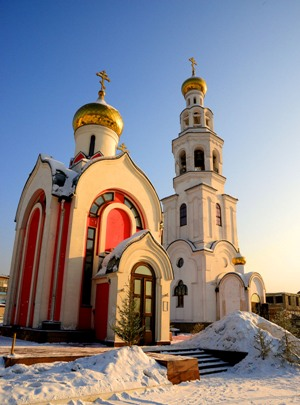
\includegraphics[width= 1\linewidth]{4a}
		\caption{\small\textit{\color{quantoan}Nhà thờ Phục sinh ở Kyzyl, Tuva (ảnh từ Internet).}}
%		\vspace*{-10pt}
	\end{figure}
\end{multicols}